\begin{frame}
	\vspace{2cm}
	\begin{center}
		{\Huge\textbf{\textcolor{copenhagenred}{Slice Sampling}}}
		\vspace{2cm}
		\vspace{1cm}

		\rule{4cm}{3pt}
	\end{center}
\end{frame}

\begin{frame}{Slice Sampling}
	\begin{block}{What is Slice Sampling?}
		A ''black-box`` auxiliary variable Markov Chain Monte Carlo (MCMC) method that
		avoids the need to tune hyperparameters. Introduced by Neal (2003).
	\end{block}

	The idea of slice sampling. 
	
	Suppose we wish to sample from a density  for a
	variable, $x$, taking values in some subset of $R^n$ . We can do this by sampling uniformly from the
	(n + 1)-dimensional region that lies under the plot of the density function.
\end{frame}

\begin{frame}{Joint and Marginal Distributions}
	This idea can be
	formalized by introducing an auxiliary real variable, $y$, and defining a joint
	distribution over $x$ and $y$ that is uniform over the region
	$U = \{ (x,y):0 < y < f (x) \}$ below the curve or surface defined
	by $f (x)$. That is, the joint density for $(x,y)$ is

	\begin{equation*}
		p(x,y) = \frac{1}{Z} \mathbf{1}_{\{0 < y < f(x)\} } 
	\end{equation*}

	where $Z = \int f(x)dx$. The marginal density for $x$ is then
	\begin{equation*}
		p(x) = \int_0^{f(x)} \frac{1}{Z} dy = \frac{f(x)}{Z}
	\end{equation*}
	which is the desired distribution. Thus, if we can sample from the joint
	distribution $p(x,y)$, we can obtain samples from the marginal distribution $p(x)$.
\end{frame}

\begin{frame}{The Slice Sampling Algorithm}
	\begin{columns}[T]
		\begin{column}{0.48\textwidth}
			\textbf{Step 1: Vertical Slice}
			\begin{itemize}
				\item Given current position $x$
				\item Sample height $y \sim \text{Uniform}(0, \pi(x))$
				\item Defines horizontal ``slice'' at height $y$
			\end{itemize}
			\textbf{Step 2: Horizontal Slice}
			\begin{itemize}
				\item Sample new $x$ uniformly from slice $S = \{x : \pi(x) \geq y\}$
			\end{itemize}	
			
			\vspace{0.2cm}
			The Challenge: In practice, sampling $S = \{ x : \pi ( x ) \geq y \}$ can be difficult!
		\end{column}
		\begin{column}{0.48\textwidth}
			\begin{center}
				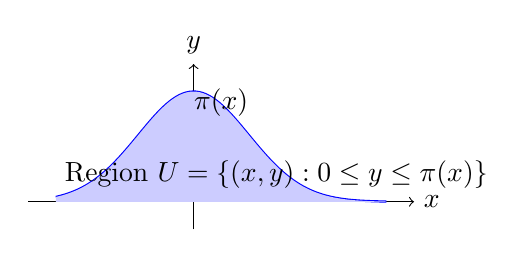
\begin{tikzpicture}[scale=0.7]
					\draw[->] (-3,0) -- (4,0) node[right] {$x$};
					\draw[->] (0,-0.5) -- (0,2.5) node[above] {$y$};
					\draw[thick,blue,domain=-2.5:3.5,smooth,samples=100] plot (\x,{2*exp(-(\x)^2/2)});
					\fill[blue!20,domain=-2.5:3.5,smooth,samples=100] plot (\x,{2*exp(-(\x)^2/2)}) -- (3.5,0) -- (-2.5,0) -- cycle;
					\node at (0.5,1.8) {$\pi(x)$};
					\node at (1.5,0.5) {Region $U = \{(x,y): 0 \leq y \leq \pi(x)\}$};
				\end{tikzpicture}
			\end{center}
			\textbf{Key Insight}:
				By alternating between sampling $y|x$ and $x|y$, we create a Markov chain that explores the space under $\pi(x)$ uniformly, with marginal distribution for $x$ being exactly $\pi(x)$
		\end{column}
	\end{columns}
\end{frame}

\begin{frame}{How to sample from $S$}
	\begin{columns}[T]
		\begin{column}{0.48\textwidth}
			\begin{block}{The Stepping Out Procedure}
				\begin{enumerate}
					\item \textbf{Create initial interval:}
					\item $L = x_t - w \cdot U$, $R = L + w$, where $U \sim \text{Uniform}(0,1)$
					\item \textbf{Step out left:}
					\item While $\pi(L) \geq y$: $L = L - w$
					\item \textbf{Step out right:}
					\item While $\pi(R) \geq y$: $R = R + w$
				\end{enumerate}
			\end{block}
		\end{column}
		\begin{column}{0.48\textwidth}
			\begin{block}{The Shrinking Procedure}
				\begin{enumerate}
					\item \textbf{Sample and shrink:}
					\item Loop: $x' \sim \text{Uniform}(L, R)$
					\item If $\pi(x') \geq y$: accept $x_{t+1} = x'$
					\item Else: shrink $[L,R]$ by setting $L = x'$ or $R = x'$
				\end{enumerate}
			\end{block}
		\end{column}
	\end{columns}

	\textbf{Adaptive Nature}: The algorithm automatically adapts to the local scale of $\pi(x)$. Wide regions are explored with large steps, narrow regions with small steps.
	Alternative procedures exist for sampling from $S$ e.g., doubling.
\end{frame}

\begin{frame}{Reversibility and Detailed Balance}

	\textbf{The geometric intuition}: Even though the stepping-out starts from different locations,
	both procedures ultimately sample uniformly from the same slice S, making the transitions symmetric.

	\vspace{0.3cm}
	The conditional transition probability $T(x_0 \rightarrow x_1 | y)$ equals:

	$P(\text{sample}\: y \vert \text{at}\: x_0) \times P(\text{sample}\: x_1 | y, \text{starting from}\: x_0)=  [1/\pi(x_0)] \times [1/|S_y|]$

	Similarly, the conditional transition probability $T(x_1 \rightarrow x_0 | y)$ equals: $[1/\pi(x_1)] \times [1/|S_y|]$

	For detailed balance, we need to show that:
	$$\pi(x_0) \cdot T(x_0 \rightarrow x_1) = \pi(x_1) \cdot T(x_1 \rightarrow x_0)$$

	% \begin{block}{1. Detailed Balance}
	% 	Let $T(x'|x)$ be the transition kernel. We need: $\pi(x) \cdot T(x'|x) = \pi(x') \cdot T(x|x')$
	% \end{block}

	The full kernel is obtained by integrating over all possible $y$:
	$$T(x_0 \rightarrow x_1) = \int_0^{\min(\pi(x_0),\pi(x_1))} \frac{1}{\pi(x_0)} \cdot \frac{1}{|S_y|} dy$$

\end{frame}

\begin{frame}{Convergence - Continued}
	\begin{block}{Irreducibility}
		No matter where we start, there's always a positive probability of sampling a
		very small $y$ value, which creates a very large slice that can connect distant
		parts of the state space, i.e. the slice is allmost the entire support of $\pi(x)$.
	\end{block}

	\begin{block}{Aperiodicity}
		$P(x \to x) > 0$ (can stay at current state) $\Rightarrow$ period = 1
	\end{block}

	\begin{block}{Ergodic Theorem}
		Since the chain is detailed balanced, irreducible and aperiodic,
		it has convergence with stationary distribution $\pi(x)$:
	\end{block}
\end{frame}

\begin{frame}{Various topics}
	\begin{itemize}
		\item How to choose initial width $w$?
		\item Extensions to Multivariate Slice Sampling. Coordinate-wise: Apply one-dimensional slice sampling to
each $x_i$ in turn. (Gibbs sampling)
		\item Elliptical Slice Sampling for Gaussian priors (Murray et al., 2010)
		\item $\pi ( x ) \propto N ( x | 0, \sigma^2 ) L ( x )$
		\item sample from prior and construct ellipse where the density on the ellipse is proportional to the likelihood
	\end{itemize}
\end{frame}
